\section{Citus}
\label{sec:citus}

\href{https://www.citusdata.com/}{Citus}~--- горизонтально масштабируемый PostgreSQL кластер. Citus использует механизм расширений PostgreSQL вместо того, что бы использовать модифицированную версию базы (как это делает <<\ref{sec:postgres-xc}~\nameref{sec:postgres-xc}>> или <<\ref{sec:postgres-xl}~\nameref{sec:postgres-xl}>>), что позволяет использовать новые версии PostgreSQL с новыми возможностями, сохраняя при этом совместимость с существующими PostgreSQL инструментами. Кластер предоставляет пользователям результаты запросов в режиме <<реального времени>> для большого и растущего обьема данных (благодаря параллелизации запросов между нодами). Примеры использования:

\begin{itemize}
  \item аналитика и вывод данных в реальном времени на графики;
  \item хранение большого набора данных для архива и создание отчетов по ним;
  \item анализ и сегментация большого обьема данных;
\end{itemize}

Нагрузки, которые требуют большой поток данных между узлами кластера, как правило, не будет хорошо работать с Citus кластером. Например:

\begin{itemize}
  \item традиционные хранилища данных с длительными и в свободном формате SQL запросами (data warehousing);
  \item множественные распределенные транзакции между несколькими шардами;
  \item запросы, которые возвращают данные по тяжелым \href{https://ru.wikipedia.org/wiki/ETL}{ETL} запросам;
\end{itemize}



\subsection{Архитектура}

На верхнем уровне Citus кластер распределяет данные по PostgreSQL экземплярам. Входящие SQL запросы затем обрабатываются паралельно через эти сервера.

\begin{figure}[ht!]
  \center{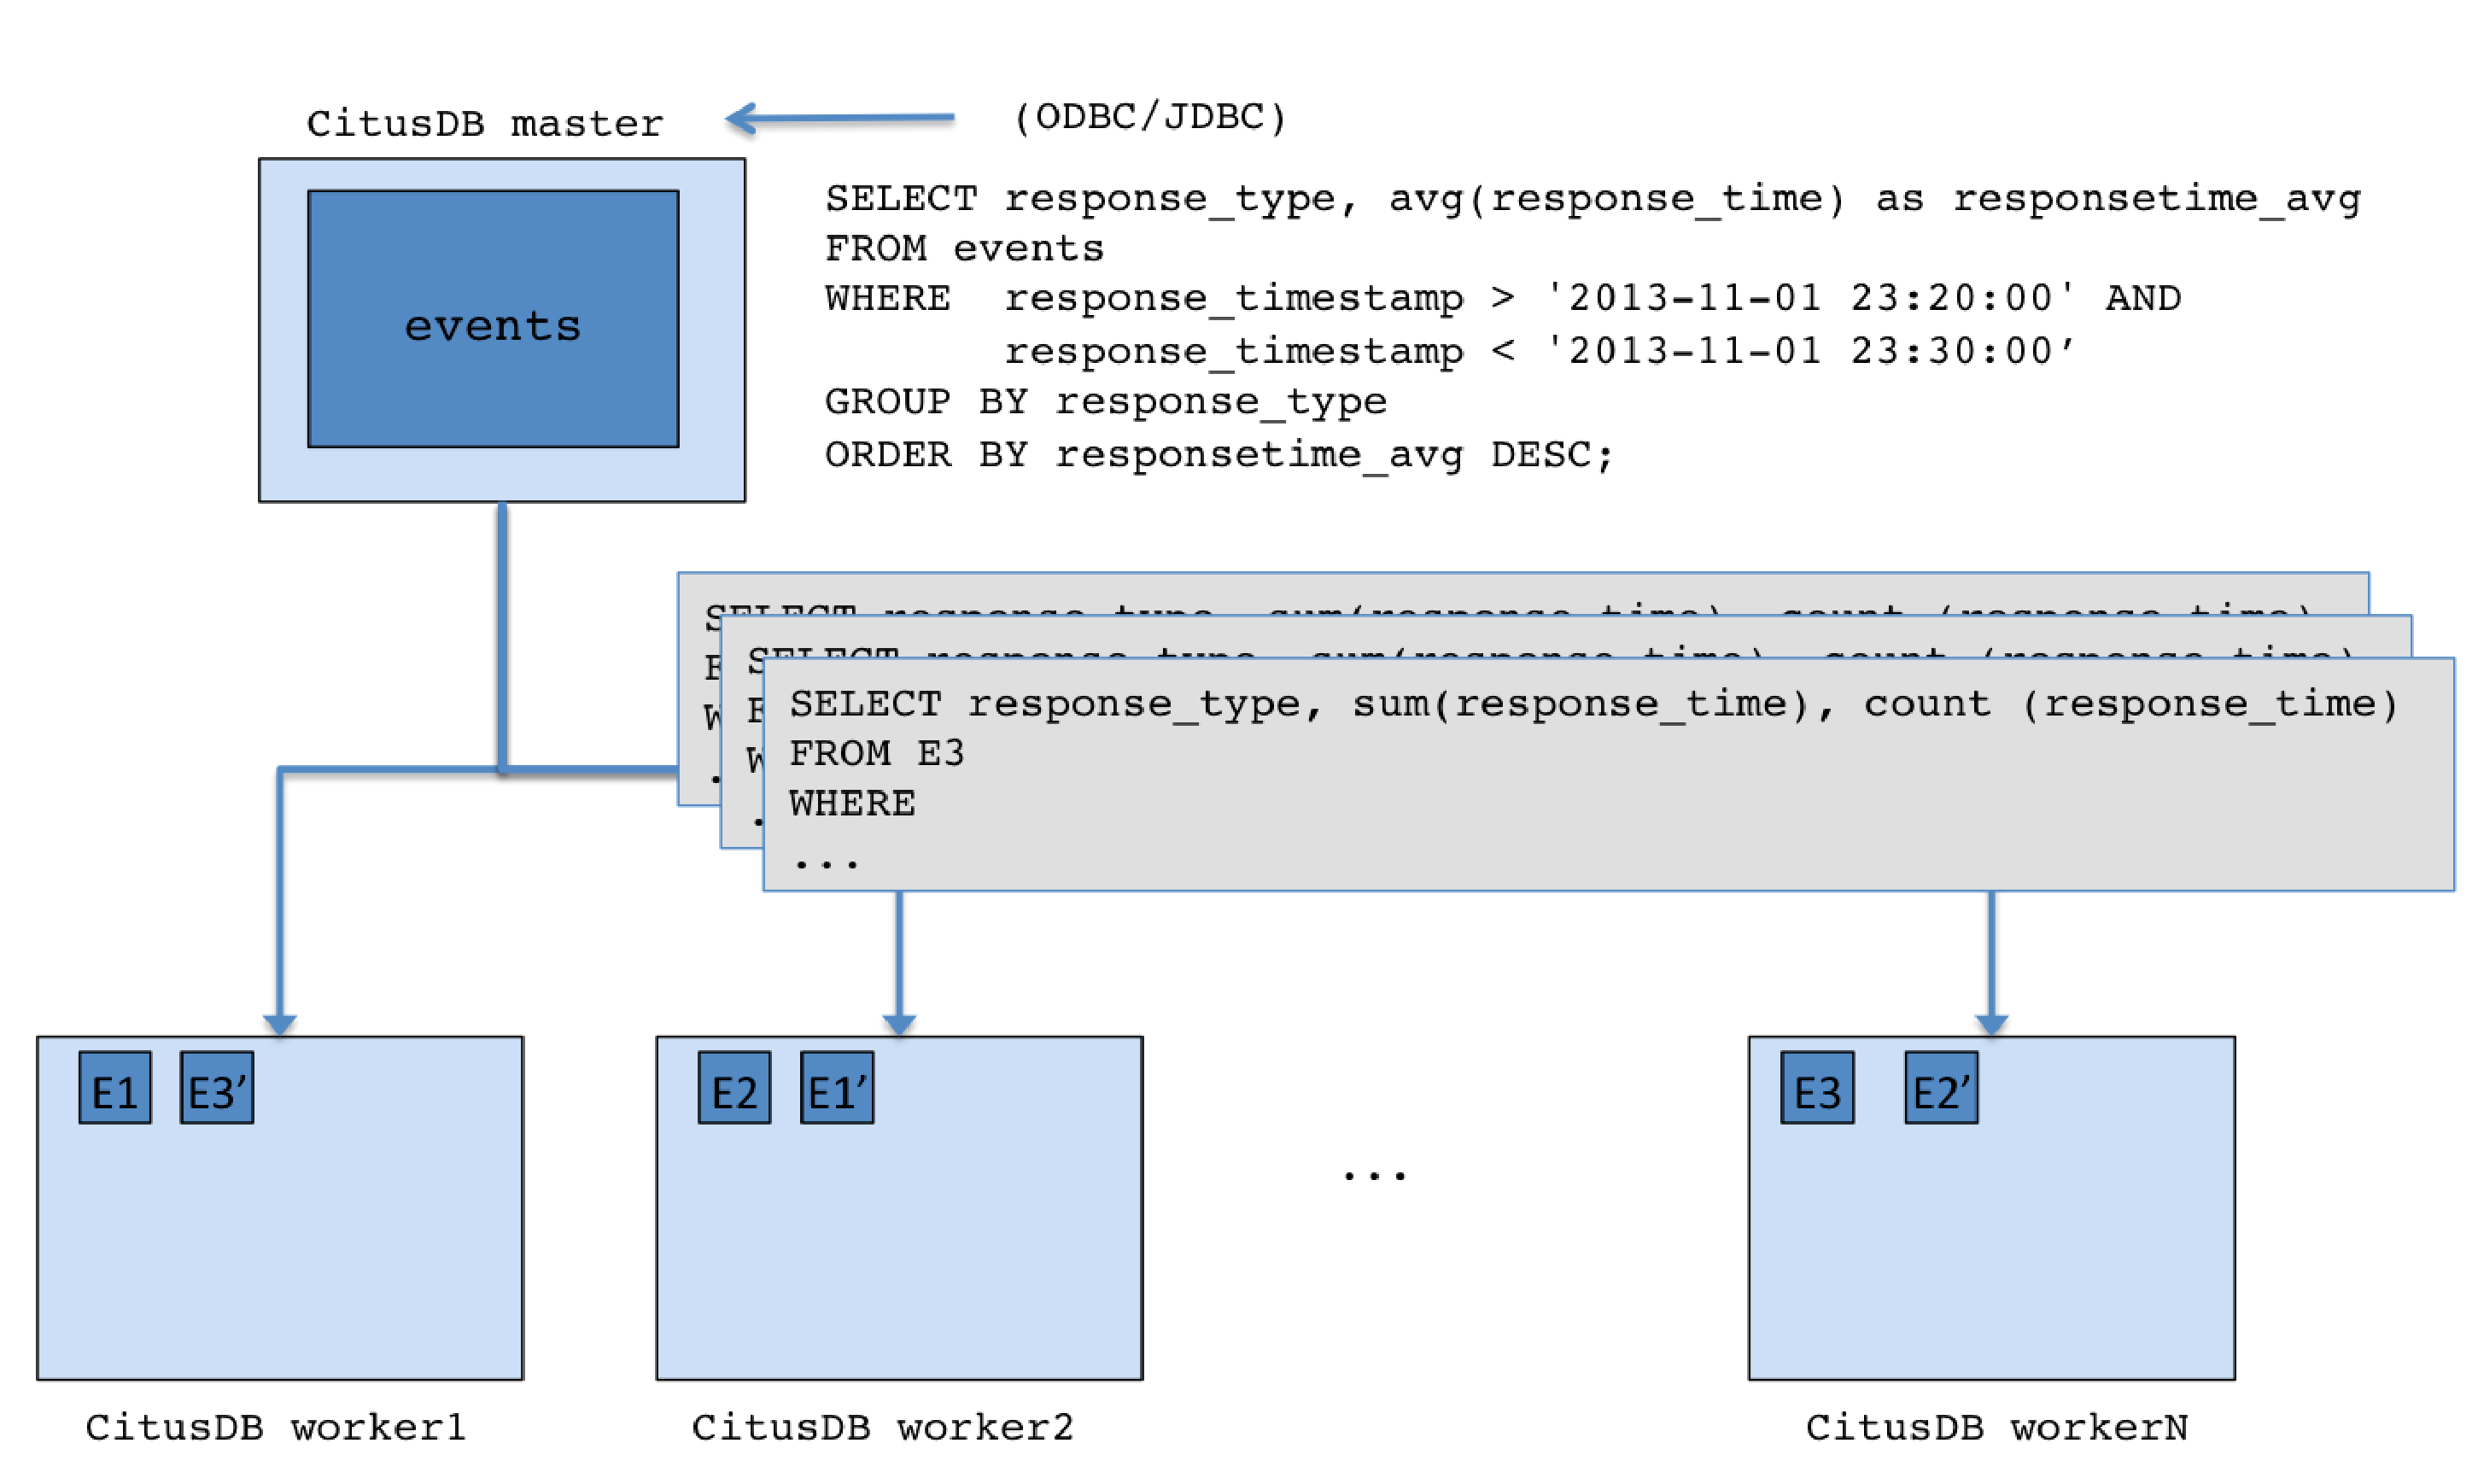
\includegraphics[width=1\textwidth]{citus-basic-arch.pdf}}
  \caption{Архитектура Citus кластера}
  \label{fig:citus_basic_arch}
\end{figure}

При разворачивании кластера один из экземпляров PostgreSQL выбирается в качестве мастер (master) ноды. Затем остальные добавляются как PostgreSQL воркеры (worker) в конфигурационном файле мастер ноды. После этого все взаимодействие с кластером ведется через мастер ноду с помощью стандартных PostgreSQL интерфейсов. Все данные распределены по воркерам. Мастер хранит только метаданные о воркерах.

Citus использует модульную архитектуру для блоков данных, которая похожа на \href{https://ru.wikipedia.org/wiki/Hadoop#HDFS}{HDFS} (Hadoop Distributed File System), но использует PostgreSQL таблицы вместо файлов. Каждая из этих таблиц представляет собой горизонтальный раздел или логический <<шард>> (shard). Каждый шард дублируется, по крайней мере, на двух воркерах (можно настроить на более высокое значение). В результате, потеря одной машины не влияет на доступность данных. Логическая архитектура шардинга в Citus также позволяет добавлять новые воркеры, чтобы увеличить пропускную способность и вычислительную мощность кластера.

Citus мастер содержит таблицы метаданных для отслеживания всех воркеров и расположение шардов базы данных на них. Эти таблицы также ведут статистику, такую как размер и минимальное/максимальное значений в шардах, которые помогают распределеннию SQL запросов Citus планировщику. Таблицы метаданных небольшие (обычно несколько мегабайт), и могут быть дублированы и быстро восстановлены, если с мастером когда-либо произойдет сбой. Подробнее про таблицах метаданных можно глянуть \href{https://docs.citusdata.com/en/latest/reference/metadata_tables.html}{в документации}.

Когда кластер получает SQL запрос, Citus мастер делит его на более мелкие фрагменты запросов, где каждый фрагмент может выполняться независимо на воркере. Это позволяет Citus распределять каждый запрос в кластере, используя вычислительные мощности всех задействованных узлов, а также отдельных ядер на каждом узле. Мастер затем поручает воркерам выполнить запрос, осуществляет контроль за их исполнением, объединяет результаты по запросам и возвращает конечный результат пользователю. Для того, чтобы гарантировать, что все запросы выполняются в масштабируемой манере, мастер также применяет оптимизации, которые сводят к минимуму объем данных, передаваемых по сети.

Citus кластер может легко переносить сбои воркеров из-за своей логической шардинг архитектуре. Если воркер терпит неудачу во время выполнения запроса, Citus завершает запрос, направляя неудачные части запроса другим воркерам, которые имеют копию данных. Если воркер находится в не рабочем состоянии (сервер упал), пользователь может легко произвести ребалансировку кластера, чтобы поддерживать тот же уровень доступности.


\subsection{Установка}

Установка Citus кластера не требует особых усилий. Для использовании в боевом окружении лучше изучить \href{https://docs.citusdata.com/en/latest/installation/production.html}{данную документиацию}. Для проверки, что кластер работает и мастер видит воркеры можно выполнить команду \lstinline!master_get_active_worker_nodes!, которая покажет список воркеров:

\begin{lstlisting}[language=SQL,label=lst:citus1,caption=Список воркеров]
postgres=# select * from master_get_active_worker_nodes();
 node_name | node_port
-----------+-----------
 localhost |      9702
 localhost |      9701
(2 rows)
\end{lstlisting}


\subsection{Распределенные таблицы}

Каждая распределенная таблица в Citus содержит стоблец, который должен быть выбран в качестве значения для распределения по шардам (возможно выбрать только один столбец). Это информирует базу данных как хранить статистику и распределять запросы по кластеру. Как правило, требуется выбрать столбец, который является наиболее часто используемым в запросах \lstinline!WHERE!. В таком случае запросы, который в фильтре используют данный столбец будут выполнятся на шардах, который выбираются по условию фильтрации. Это помогает значительно уменьшить количество вычислений на шардах.

Следующим шагом после выбора столбца на распределения будет определение правильного метода распределения данных в таблицу. В целом, существует два шаблона таблиц: распределенные по времени (время создания заказа, запись логов, прочее) и распределение по идентификатору (ID пользователя, ID приложения, прочее). Citrus поддерживает оба метода распределения: append и hash соответственно.

Append метод подходит для таблиц, в которые записываются данные по времени (упорядочены по времени). Такой тип таблиц отлично справляется с запросами, которые использут фильтры с диапазонами значений по распределенному столбцу (\lstinline!BETWEEN x AND y!). Это обьясняется тем, что мастер хранить диапазоны значений, которые хранятся на шардах и планировщик может эффективно выбирать шарды, которые содержат данные для SQL запроса.

Hash метод распределения подходит для неупорядоченного столбца (user UUID) или по данным, которые могут записываться в любом порядке. В таком случае Citus кластер будет хранить минимальные и максимальные значения для хеш функций на всех шардах. Это модель лучше подходит для SQL запросов, включающих фильтры на основе равенства по колонке распределения (\lstinline!user_uuid='a0eebc99-9c0b-4ef8-bb6d-6bb9bd380a11'!).


\subsubsection{Hash распределение}

Для примера создадим и распределим таблицу по hash методу.

\begin{lstlisting}[language=SQL,label=lst:citus_hash1,caption=Создание таблицы]
# CREATE TABLE github_events
(
    event_id bigint,
    event_type text,
    event_public boolean,
    repo_id bigint,
    payload jsonb,
    repo jsonb,
    actor jsonb,
    org jsonb,
    created_at timestamp
);
\end{lstlisting}

Далее укажем Citus кластеру использовать \lstinline!repo_id! с hash распределением для \lstinline!github_events! таблицы.

\begin{lstlisting}[language=SQL,label=lst:citus_hash2,caption=Создание hash распределения]
# SELECT master_create_distributed_table('github_events', 'repo_id', 'hash');
\end{lstlisting}

И создадим шарды для таблицы:

\begin{lstlisting}[language=SQL,label=lst:citus_hash2,caption=Создание шардов]
# SELECT master_create_worker_shards('github_events', 16, 1);
\end{lstlisting}

Данный метод принимает два аргумента в дополнение к имени таблицы: количество шардов и коэффициент репликации. Этот пример позволит создать в общей сложности шестнадцать шардов, где каждый будет владеть частью символического пространства хэша, а данные будут реплицироватся на один воркер.

Далее мы можем заполнить таблицу данными:

\begin{lstlisting}[language=Bash,label=lst:citus_hash3,caption=Загрузка данных]
$ wget http://examples.citusdata.com/github_archive/github_events-2015-01-01-{0..5}.csv.gz
$ gzip -d github_events-2015-01-01-*.gz
\end{lstlisting}

\begin{lstlisting}[language=SQL,label=lst:citus_hash4,caption=Загрузка данных]
# \COPY github_events FROM 'github_events-2015-01-01-0.csv' WITH (format CSV)
# INSERT INTO github_events VALUES (2489373118,'PublicEvent','t',24509048,'{}','{"id": 24509048, "url": "https://api.github.com/repos/SabinaS/csee6868", "name": "SabinaS/csee6868"}','{"id": 2955009, "url": "https://api.github.com/users/SabinaS", "login": "SabinaS", "avatar_url": "https://avatars.githubusercontent.com/u/2955009?", "gravatar_id": ""}',NULL,'2015-01-01 00:09:13');
\end{lstlisting}

Теперь мы можем обновлять и удалять данные с таблицы:

\begin{lstlisting}[language=SQL,label=lst:citus_hash5,caption=Изменение данных]
# UPDATE github_events SET org = NULL WHERE repo_id = 24509048;
# DELETE FROM github_events WHERE repo_id = 24509048;
\end{lstlisting}

Для работы \lstinline!UPDATE! и \lstinline!DELETE! запросов требуется, что бы он <<затрагивал>> один шард. Это означает, что условие \lstinline!WHERE! должно содержать условие, что ограничит выполнение запроса на один шард по распределенному столбцу. Для обновления или удаления данных на нескольких шардах требуется использовать команду \lstinline!master_modify_multiple_shards!:

\begin{lstlisting}[language=SQL,label=lst:citus_hash6,caption=Изменение данных на нескольких шардах]
# SELECT master_modify_multiple_shards(
  'DELETE FROM github_events WHERE repo_id IN (24509048, 24509049)');
\end{lstlisting}

Для удаления таблицы достаточно выполнить \lstinline!DROP TABLE! на мастере:

\begin{lstlisting}[language=SQL,label=lst:citus_hash7,caption=Удаление таблицы]
# DROP TABLE github_events;
\end{lstlisting}


\subsubsection{Append распределение}

Для примера создадим и распределим таблицу по append методу.

\begin{lstlisting}[language=SQL,label=lst:citus_append1,caption=Создание таблицы]
# CREATE TABLE github_events
(
    event_id bigint,
    event_type text,
    event_public boolean,
    repo_id bigint,
    payload jsonb,
    repo jsonb,
    actor jsonb,
    org jsonb,
    created_at timestamp
);
\end{lstlisting}

Далее укажем Citus кластеру использовать \lstinline!created_at! с append распределением для \lstinline!github_events! таблицы.

\begin{lstlisting}[language=SQL,label=lst:citus_append2,caption=Создание hash распределения]
# SELECT master_create_distributed_table('github_events', 'created_at', 'append');
\end{lstlisting}

После этого мы можем использовать таблицу и загружать в нее данные:

\begin{lstlisting}[language=SQL,label=lst:citus_append3,caption=Загрузка данных]
# SET citus.shard_max_size TO '64MB';
# \copy github_events from 'github_events-2015-01-01-0.csv' WITH (format CSV)
\end{lstlisting}

По умолчанию команда \lstinline!\copy! требует два конфигурационных параметра для работы: \lstinline!citus.shard_max_size! и \lstinline!citus.shard_replication_factor!.

\begin{itemize}
  \item \lstinline!citus.shard_max_size! параметр указывает максимальный размер шарда при использовании команды \lstinline!\copy! (1Гб по умолчанию). Если файл больше данного параметра, то команда автоматически разобьет файл по нескольким шардам;
  \item \lstinline!citus.shard_replication_factor! параметр количество воркеров, на которые шарды будут реплицироватся (2 по умолчанию);
\end{itemize}

По умолчанию, команда \lstinline!\copy! создает каждый раз новый шард для данных. Если требуется добавлять данные в один и тот же шард, существуют команды \lstinline!master_create_empty_shard!, которая вернет идентификатор на новый шард и команда \lstinline!master_append_table_to_shard! для добавления данных в этот шард по идентификатору.

Для удаления старых данных можно использовать команду \lstinline!master_apply_delete_command!, которая удаляют старые шарды, которые попадают в переданное условие на удаление:

\begin{lstlisting}[language=SQL,label=lst:citus_append4,caption=Удаление старых шардов]
# SELECT * from master_apply_delete_command('DELETE FROM github_events WHERE created_at >= ''2015-01-01 00:00:00''');
 master_apply_delete_command
-----------------------------
                           3
(1 row)
\end{lstlisting}

Для удаления таблицы достаточно выполнить \lstinline!DROP TABLE! на мастере:

\begin{lstlisting}[language=SQL,label=lst:citus_append5,caption=Удаление таблицы]
# DROP TABLE github_events;
\end{lstlisting}



\subsection{Ребалансировка кластера}

Логическая архитектура шардинга Citus позволяет маштабировать кластер без каких-либо простоев (no downtime!). Для добавления нового воркера достаточно добавить его в \lstinline!pg_worker_list.conf! и вызвать на мастере \lstinline!pg_reload_conf! для загрузки новой конфигурации:

\begin{lstlisting}[language=SQL,label=lst:citus_balance1,caption=Загрузка новой конфигурации]
# SELECT pg_reload_conf();
\end{lstlisting}

После этого Citus автоматически начнет использовать данный воркер для новых распределенных таблиц. Если требуется ребалансировать существующие таблицы на новый воркер, то для этого есть команда \lstinline!rebalance_table_shards!, но, к сожалению, она доступна только в Citus Enterprise (платное решение).


\subsection{Ограничения}

Модель расширения PostgreSQL в Citus позволяет использовать доступные типы данных (JSON, JSONB, другие) и другие расширения в кластере. Но не весь спектр SQL запросов доступен для распределенных таблиц. На текущий момент распределенные таблицы не поддерживают:

\begin{itemize}
  \item Оконные функцие (window functions);
  \item Общие табличные выражения (CTE);
  \item \lstinline!UNION! операции (\lstinline!UNION/INTERSECT/EXCEPT!);
  \item Транзакционная семантика для запросов, которые распределены по нескольким шардам;
\end{itemize}



\subsection{Заключение}

Citus кластер достаточно гибкое и мощное решение для горизонтального масштабирования PostgreSQL. Зрелость данного решения показывает его использование такими игроками на рынке, как CloudFlare, Heap и многими другими.
